\documentclass[a4paper,12pt,oneside,openright,onecolumn, fleqn, final,titlepage,ngerman]{scrreprt}

% Gliederungsebenen:
% \part{}
% \chapter{}
% \section{}
% \subsection{}
% \subsubsection{}
% \paragraph{}
% \subparagraph{}

% Package definitions
\usepackage[ngerman]{babel}
\usepackage[utf8]{inputenc}

% package to control enumerations
\usepackage{enumerate}

% package to make the shorting table
\usepackage{longtable}
\renewcommand{\arraystretch}{1.5}

% use graphix
\usepackage{graphicx}

% for mathematical formula
\usepackage{amsmath}

% flushleft for caption
\usepackage{caption}

% use colors
\usepackage{color}
\definecolor{orange}{rgb}{1,0.784,0}
\definecolor{gray}{rgb}{0.5,0.5,0.5}

% package for killing borders at title page
\usepackage{geometry}

% Quotations
% \usepackage[numbers]{natbib}
\usepackage{multibib}
% \bibliographystyle{alphadin}

% other useful packages
\usepackage{tabularx}

% syntax highlighting
\usepackage{scrhack}		% makes a warning disappearing, but does dirty things!

% for links, LOAD AT LAST!
\usepackage[colorlinks,
pdfpagelabels,
pdfstartview = FitH,
bookmarksopen = true,
bookmarksnumbered = true,
linkcolor = black,
plainpages = false,
hypertexnames = false,
citecolor = black] {hyperref}

% set bibliographies
\newcommand{\refver}{Bibliography}
\newcommand{\webver}{Index of web address}
\newcites{Refs,Urls}{\refver, \webver}

% disable indents for new paragraphs
\setlength{\parindent}{0cm}

% set header/footer
\usepackage{scrpage2}
\pagestyle{scrheadings}
% \setkomafont{pageheadfoot}{}		% set heading not italic
\automark{chapter}

\usepackage{tocloft}
\renewcommand{\cftfigpresnum}{Abb. }
\renewcommand{\cftfigaftersnum}{:}
\settowidth{\cftfignumwidth}{Abb. 8.88\quad}

% set new symbol for itemize-environment
\renewcommand{\labelitemi}{--}

% set depth of toc (depth=3, starts at 0!)
\setcounter{tocdepth}{2}

% important commands
\newcommand{\parag}{\\[2ex]}
\newcommand{\zB}{z.\,B.}
\newcommand{\abkEntry}[2]{\textbf{#1} & #2\\}
\newcommand{\imgCaption}[2]{\caption[#1]{#1 (\textit{Quelle:} #2)}}			% to define the sources of images

% set some constants
\newcommand{\calcag}{Berechnungsagent}
\newcommand{\coordag}{Koordinationsagent}
\newcommand{\repag}{Darstellungsagent}
\newcommand{\numag}{Numerikagent}
\newcommand{\iteag}{ITE-Agent}

\renewcommand{\ttdefault}{pcr}
% Document
\begin{document}
\bibliographystyleRefs{plaindin}
	% setting roman counter for toc,...
	\pagenumbering{Roman}

	% title page
	\begin{titlepage}
		% kill borders for title page
		\newgeometry{
			left=1cm,
			right=1cm,
			top=2cm,
			bottom=1cm,
			bindingoffset=5mm
		}

		\begin{center}
			\begin{tabularx}{\textwidth}{rXcXl}
				\begin{tabular}{c}
\includegraphics[keepaspectratio=true,height=0.15\textwidth]{res/unilogo.png} \end{tabular} & &
				\large\begin{tabular}{c}
					University of Stuttgart\\
					Institute for Theory of Electrical Engineering\\
					Prof. Dr. techn. Wolfgang M. Rucker
				\end{tabular}
				& & \begin{tabular}{c} 
\includegraphics[keepaspectratio=true,height=0.15\textwidth]{res/itelogo.png} \end{tabular}
			\end{tabularx}
	
			\vspace{20ex}

			{\Large\scshape Master thesis}
	
			\vspace{15ex}
	
			{\huge\bfseries Web based Visualization}
	
			\vspace{26ex}
	
			{\Large Nan Zhao}
	
			\vspace{23ex}
	
			\begin{tabbing}
				Abgabe der Ausarbeitung: \quad \= Dipl.-Ing. Matthias Jüttner\kill\\
				Betreuer: \> Dr.-Ing. Matthias Jüttner\\[0.5ex]
				Beginn der Arbeit: \> 01.02.2017\\[0.5ex]
				Abgabe der Ausarbeitung: \> 24.07.2017
			\end{tabbing}
		\end{center}
	\end{titlepage}

	% restore borders for rest of document
	\restoregeometry
	\newgeometry{bindingoffset=5mm}		% set offset for binding the whole  later

	% begin with text on the next odd page
	\thispagestyle{empty}
	\cleardoublepage

	% preface
	\chapter*{Erklärung}
	\addcontentsline{toc}{chapter}{Erklärung}
	Hiermit erkläre ich,

	\begin{itemize}
		\item dass ich die vorliegende Arbeit selbstständig verfasst habe,
		\item dass ich keine anderen als die angegebenen Quellen und alle wörtlich oder sinngemäß aus anderen Werken übernommenen Aussagen als solche gekennzeichnet habe,
		\item dass die eingereichte Arbeit weder vollständig noch in wesentlichen Teilen Gegenstand eines anderen Prüfungsverfahrens ist,
		\item dass ich die Arbeit noch nicht veröffentlicht habe,
		\item dass das elektronische Exemplar mit diesem Exemplar übereinstimmt.
	\end{itemize}

	\bigskip

	Stuttgart, den 24.07.2017

	% abstract
	\chapter*{Abstract}
\addcontentsline{toc}{chapter}{Abstract}

	

	% table of contents
	\clearpage		% flush page before printing toc -> toc to new page
	\tableofcontents
% 	\addcontentsline{toc}{chapter}{\contentsname}		% add toc to toc ;)
	
	% set new page numbering
	\pagenumbering{arabic}
	
	
	%%%%%%%%%%%%%%% Start including your chapters below %%%%%%%%%%%%%
	\include{tex_contents/Introduction}
	\chapter{Visualization System}
In this chapter the system architecture and corresponding components will be introduced. This chapter emphasizes on depicting the whole picture of the solution, some specific technical detail will be represented in the later chapters.

\section{System architecture}

The visualization system is to display the COMSOL's plots in the web application. To accomplish the goal, the system architecture in fig. 1 is needed.

\begin{figure}[htb]
  \centering
  \includegraphics[width=.9\textwidth]{Assets/System_architecture}
  \caption{System architecture}
\end{figure}

To render the graphics in the web client, the source data need to be extracted and converted at first. COMSOL provides the COMSOL Java API(CJAPI) to handle with its mph file. To use the CJAPI, a Java application is needed. The Java application can access into the model object and extract the meta information and binary data of plots, then export the required data separately into JavaScript Object Notation(JSON) file and binary file. Via a Secure File Transfer Protocol(SFTP), the files are committed to the web server. As the back-end, web server provides the web application and all the necessary data for visualization. The web server is built by Node.js, which is based on Google's JavaScript run-time environment. Its event-driven architecture and asynchronous I/O capability bring about good performance while loading large volume data. To meet the needs of dynamic reload of plots' data, a bidirectional connection protocol WebSocket is used between web server and web client. Since that web client runs on various browsers and devices, the compatibility must be considered. The web client is responsive design for both mobile and desktop devices and a universal UI(User Interface) is built with HTML5 standard and display the visualization results. Besides, user interaction is also supported for post-processing with the rendered graphics.

\section{Data structure of COMSOL numerical results}

 
	\chapter{Data Extraction and Conversion}
\section{Data-structure of COMSOL file}
\section{Data-format after conversion}
	\chapter{Rendering using WebGL}

\begin{figure}[htb]
  \centering
  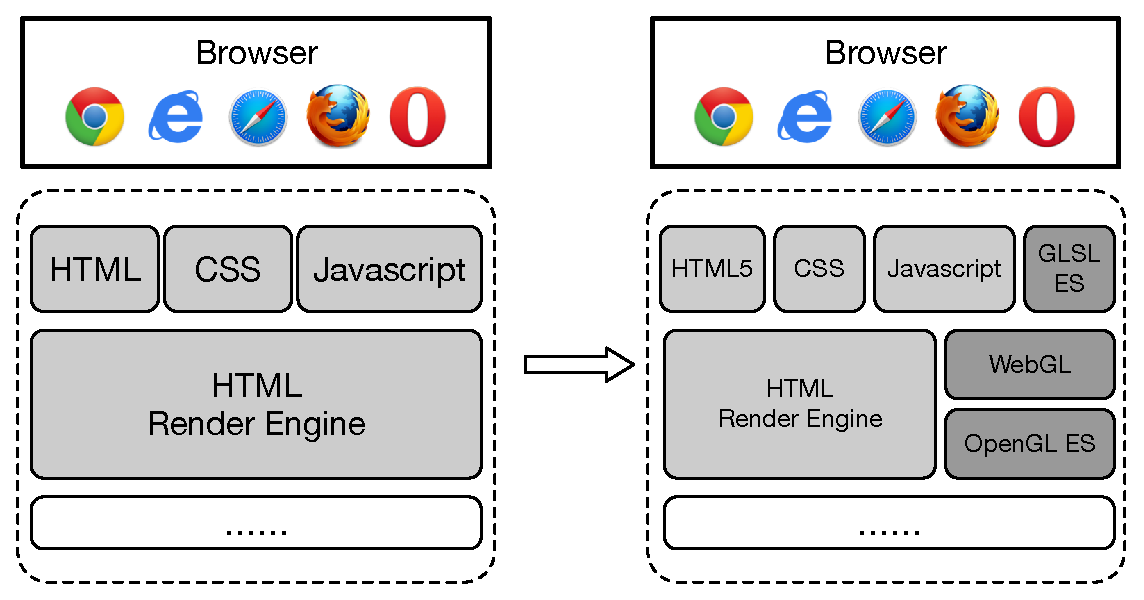
\includegraphics[width=.9\textwidth]{Assets/WebGL_HTML5}
  \caption{WebGL}
  \label{fig:ZF_MMSE_detector}
\end{figure}

\section{WebGL graphics pipeline}
\section{2D translation, rotation, scale and matrix math}
\section{3D Orthographic, Perspective, Cameras}
\section{Rendering text using sprites}
	\chapter{Virtual Reality}
	\chapter{Conclusion}
	% % creating appendix
	\appendix
	\chapter{Datenmanagement}
	Dieses Kapitel erläutert einige bedeutende Aspekte der Implementierung des \repag{}en. Diese sind sehr speziell und werden daher nur benötigt, wenn der Quelltext verstanden werden will.
	
	\section{Text-Level}\label{kap_textlevels}
	Da die Konsole eine formatierte Ausgabe erlaubt, wurden sogenannte \emph{Text-Level} eingeführt. Diese lauten (von wichtig zu unwichtig):
	
	\begin{enumerate}
		\item \emph{Fatal}: Das Problem, welches diese Nachricht verursacht, bringt das Programm zum Absturz.
		\item \emph{Error}: Dieses Problem kann nicht ignoriert werden. Das Programm läuft dennoch fort.
		\item \emph{Warning}: Das aufgetretene Problem kann ignoriert werden.
		\item \emph{Information Important}: Der Text beinhaltet eine wichtige Information für den Benutzer.
		\item \emph{Information Casual}: Der Text beinhaltet eine beiläufige Information für den Benutzer, welche dieser nicht unbedingt benötigt.
		\item \emph{Debug}: Der Text dient ausschließlich als Debug-Information. Der Benutzer sollte diese Information nicht sehen.
		\item \emph{Unknown}: Falls kein Text-Level definiert ist oder sonstige Fehler bei dessen Dekodierung auftreten.
	\end{enumerate}
	
	\section{Wichtige Klassen}\label{kap_impCl}
	\paragraph{reportagent.stats.Parameter}
	Repräsentiert einen Datensatz mit sämtlichen Informationen, die zur Darstellung eines Prozessparameters erforderlich sind, \zB{} den Diagramm-Typ. Das zur Klasse zugehörige Attribut \emph{parameterID} definiert klar den Typ des Prozessparameters, \zB{} Fortschritt.\parag{}
	\emph{Hinweis:} Dieses Attribut darf keinesfalls mit dem Attribut \emph{type} verwechselt werden, welches den \emph{Diagramm-Typ} spezifiziert, also \zB{} ein XY-Chart.

	\paragraph{reportagent.stats.ParameterMap}
	Abstrakte Klasse, die Informationen über einzelne Parametertypen enthält, beispielsweise das X-Achsen-Label des Parameters \emph{PCStatus}.

	\paragraph{reportagent.ProtocolRA}
	Interface, welches Konstanten beinhaltet. Diese definieren das Übertragungsprotokoll (siehe Kapitel \ref{kap_protocol}).

	\section{Das Übertragungsprotokoll}\label{kap_protocol}
	Übertragen werden müssen folgende Kommandos:

	\paragraph{REGISTER\_PARAMETER}
	Befehl zur Registrierung eines neuen Prozessparameters beim \repag{}en. Es wird erwartet, dass in der ACLMessage als \emph{ContentObject} ein Objekt des Typs \emph{Parameter} vorliegt.

	\paragraph{UNREGISTER\_PARAMETER}
	Befehl zum Löschen eines Prozessparameters. Wieder wird als \emph{ContentObject} ein Objekt vom Typ Parameter erwartet.

	\paragraph{UPDATE\_PARAMETER}\label{kap_UpdateMsg}
	Befehl zum Update eines Prozessparameters. Die Syntax lautet:

	\begin{lstlisting}[caption={Syntax UPDATE\_PARAMETER},label={lst_syntax_datentag}]
		<parameterID>;<Daten>
	\end{lstlisting}

	wobei der Tag \textit{Daten} frei spezifiziert werden darf. Der Code zur Interpretation dieser Zeile findet sich dabei in der Klasse \emph{reportagent.""behaviours.""Update"-Msg"-Handler}.

	\section{Austausch der Daten}\label{kap_dataman_austausch}
	Dieser Teil beschreibt die Implementierung des Datentransfers zwischen den Agenten. Diese ist sehr spezifisch und bezieht sich direkt auf die in Kapitel \ref{kap_existingPlatform} vorgestellte Beispielplattform, in die der \repag{} eingebettet ist.
	
	\subsection{Sendeseite}
	Für die Verwaltung der Daten ist der \numag{} mit der Klasse \emph{numericagent.InformationManager} ausgestattet. Die Klasse \emph{InformationManager} besitzt die Methode \emph{addParameter(\ldots)}, die den \repag{}en über einen neuen Prozessparameter informiert. Ferner besitzt der \emph{InformationManager} die Methode \emph{update(\ldots)}, die zuerst \emph{addParameter(\ldots)} aufruft, wenn nicht bereits geschehen. Anschließend wird der \repag{} über die neuen Daten informiert.\parag{}
	Da der \calcag{} von \numag{} erbt, steht ihm diese Klasse ebenfalls zur Verfügung. Zu beachten ist, dass im Design davon ausgegangen wurde, dass es von dieser Klasse nur ein Objekt gibt, dies jedoch nicht sichergestellt wurde. Hintergrund ist, dass es mehrere Instanzen des \repag{}en geben kann. Weiter läuft man bei der Programmierung keine Gefahr, mehrere Instanzen der Klasse \emph{InformationManager} zu erzeugen.

	\subsection{Empfangsseite}
	Die Parameter, die neu registriert werden, werden in dem \repag{}en hinterlegt. In der GUI wird ein neuer Tab mit dem entsprechenden Parameter angelegt. Zu beachten ist, dass ein \repag{} mehrere \numag{}en kennen kann und jeder \numag{} mehrere Parameter besitzen kann. Dies ist in der Datenstruktur zur Speicherung der Parameter berücksichtigt, es ergibt sich das Klassendiagramm aus Abbildung \ref{repag_params}.
	\begin{figure}[ht]
		\centering
		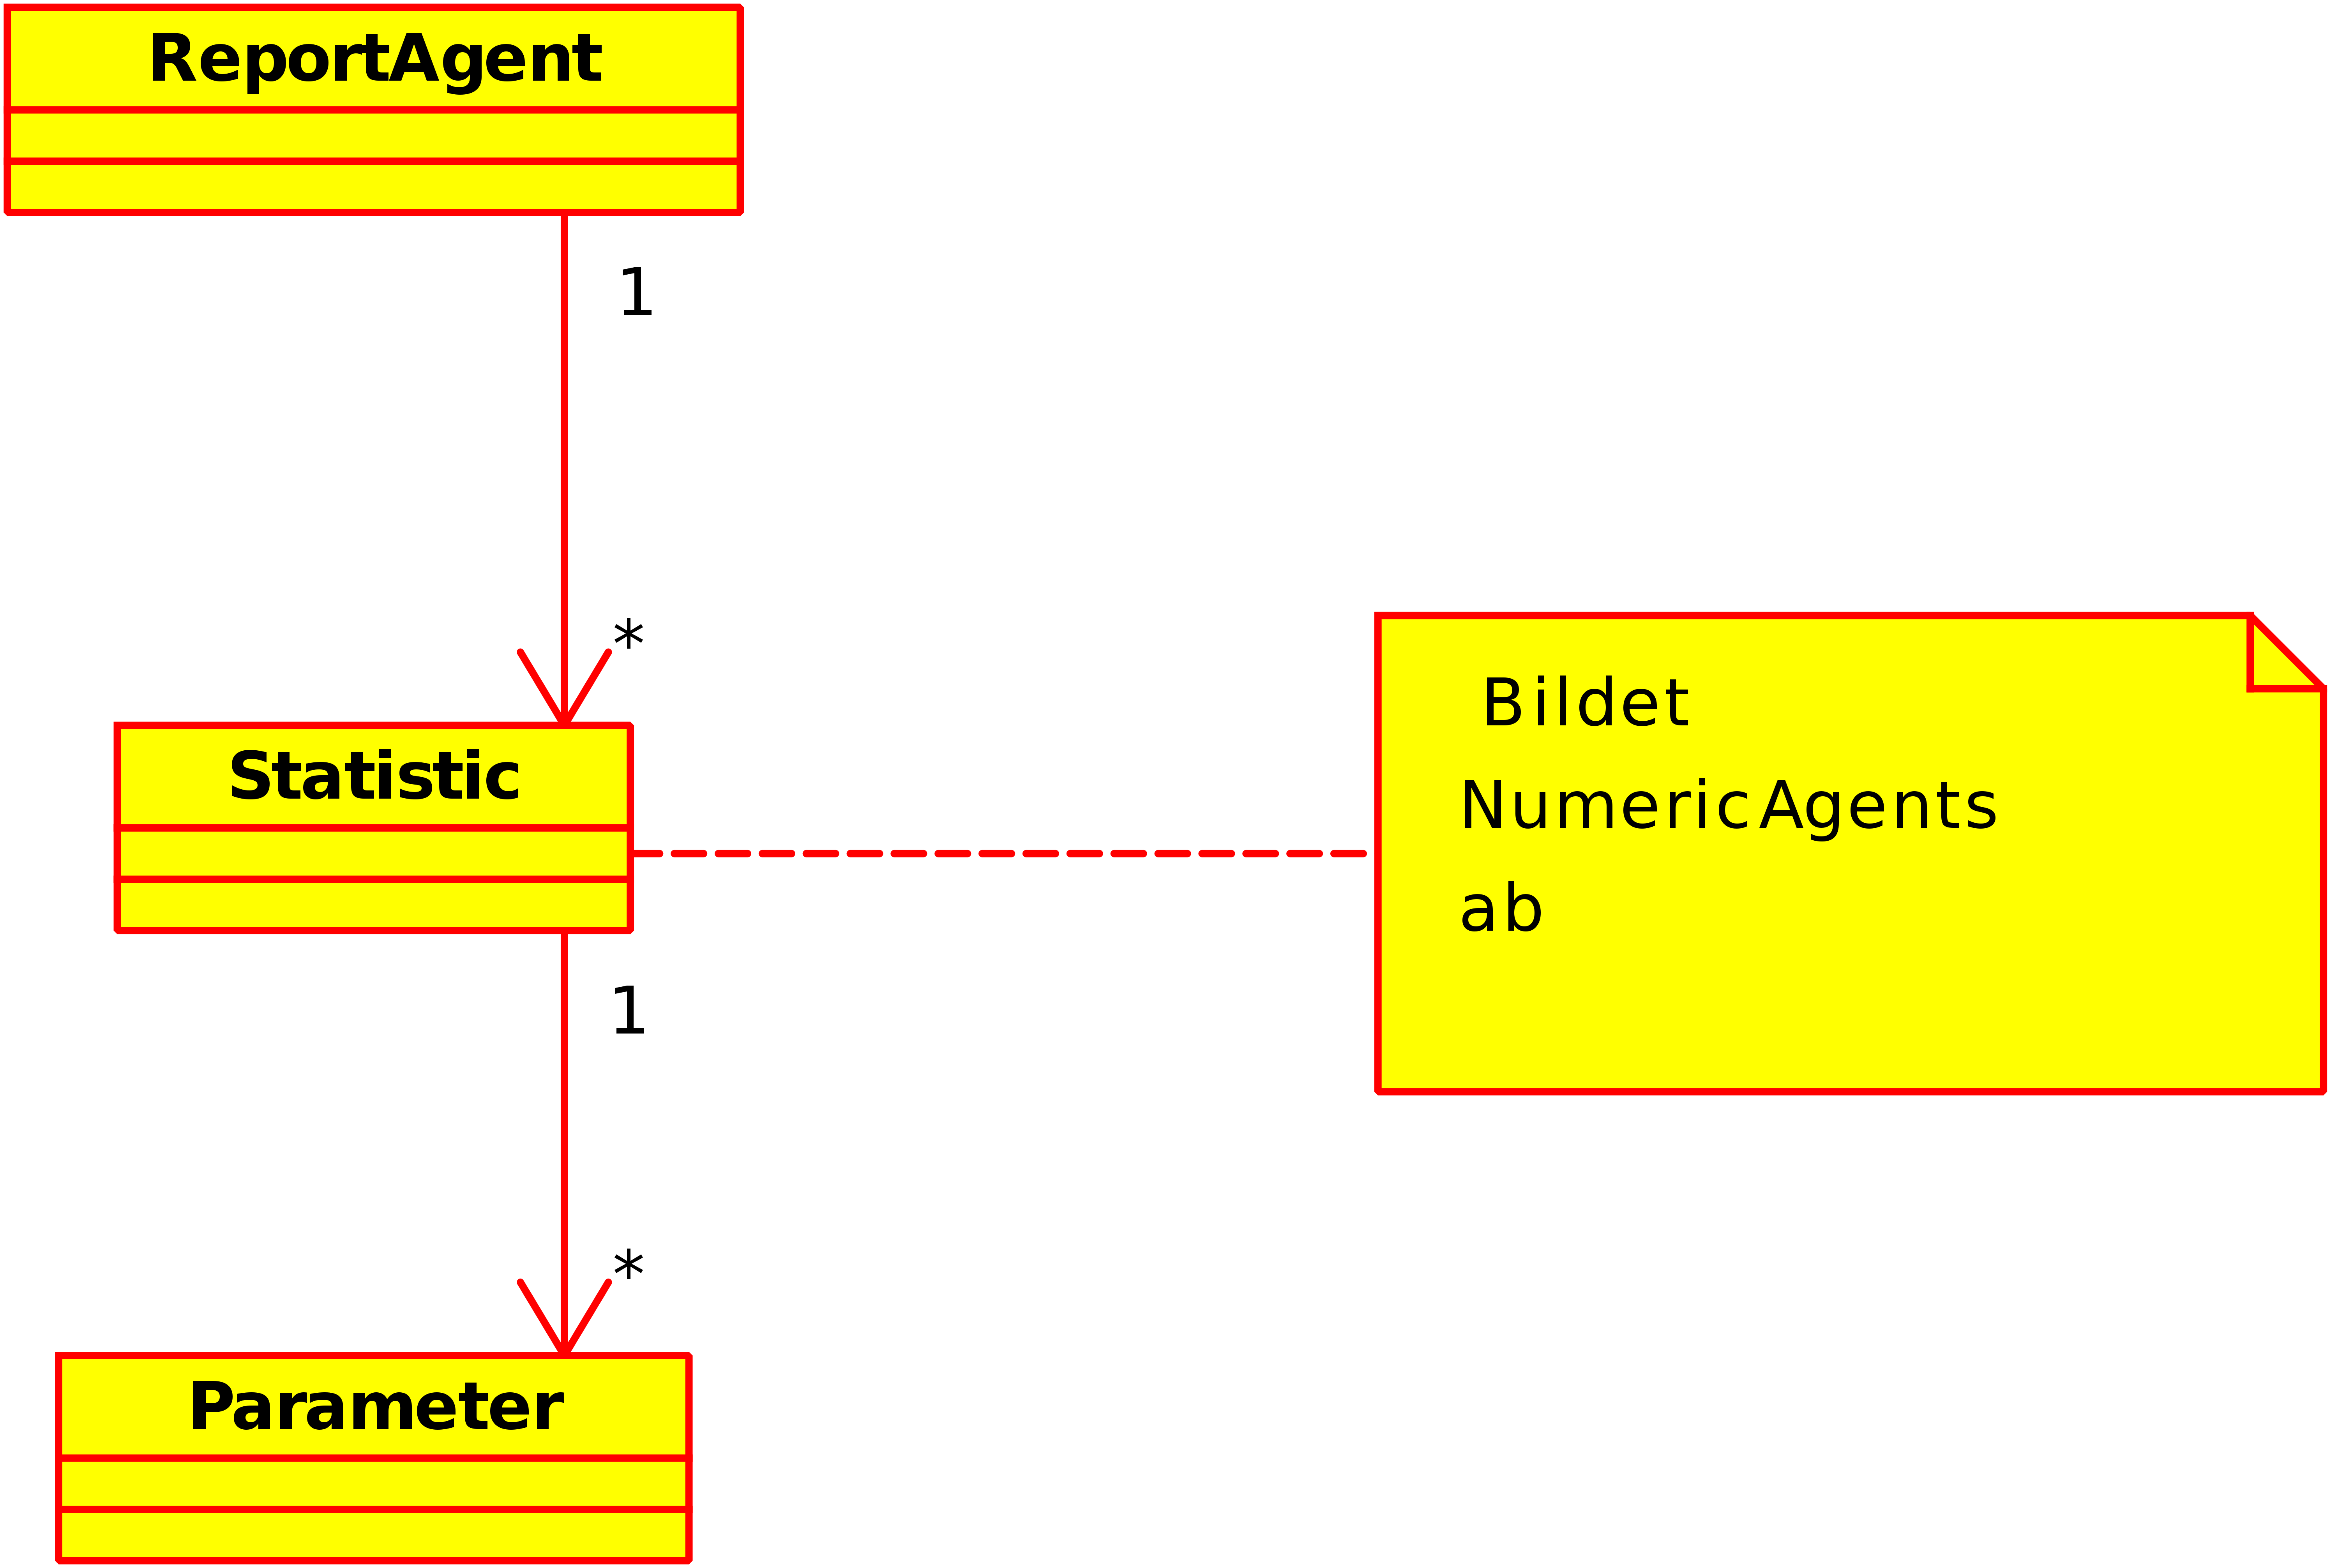
\includegraphics[keepaspectratio=true, width=\textwidth]{res/Klassendiagramm_ReportAgent_Parameterverwaltung.png}
		\caption{Parameterverwaltung des \repag{}en}
		\label{repag_params}
	\end{figure}\parag{}
	Wird nun ein neues Datum empfangen, so wird ein neuer Parameter registriert oder ein bestehender aktualisiert. Die GUI aktualisiert sich in diesem Fall automatisch.
	
	\chapter{Hinzufügen von Prozessparametern}\label{kap_AddParameter}
	Für das nachträgliche Hinzufügen von Parametern in das System müssen lediglich wenige Stellen im Programmtext bearbeitet werden. Diese werden im Folgenden kurz vorgestellt. Da dieses Kapitel als Programmieranleitung gedacht ist, wird für dessen Verständnis Zugang und Verständnis des Quelltextes vorausgesetzt.
	
	\section{Weiterleitung an den \repag{}en}
	Es wird davon ausgegangen, dass die Daten bereits abrufbar sind. Diese müssen an den \repag{}en übergeben werden. Dies geschieht durch die Klasse \emph{numericagent.InformationManager} mit der Methode \emph{addParameter(\ldots)}. Diese ist überladen (siehe \lstlistingname{} \ref{lst_InfoMgr_addParam}).
	\begin{lstlisting}[caption={Auszug aus numericagent.InformationManager},label={lst_InfoMgr_addParam}]	
public void addParameter(Parameter p) {
	...
}

public void addParameter(int paramID) {
	addParameter(new Parameter(paramID));
}
	\end{lstlisting}
	In der einen Version erwartet sie einen Parameter vom Typ \emph{reportagent.stats.Pa\-ra\-me\-ter}, in der anderen einen Parameter vom primitiven Typ \emph{Integer}. Dabei erzeugt die Methode mit dem primitiven Parameter ein neues \emph{Parameter}-Objekt und übergibt dieses an die andere Methode. Obwohl ein Fehlerfall nicht über\-prüf\-bar ist, kann davon ausgegangen werden, dass nach Aufruf dieser Methode das \emph{Parameter}-Objekt korrekt an \repag{} übergeben wurde. Aufgetretene Fehler wird die \emph{update(\ldots)}-Methode beheben.
	
	\section{Parameter}
	Um die \emph{addParameter(\ldots)}-Methode des \emph{InformationManagers} aufrufen zu kön\-nen, wird mindestens eine \emph{parameterID} benötigt (siehe \lstlistingname{} \ref{lst_InfoMgr_addParam}). Diese sollte in der Klasse \emph{Parameter} als Konstanten definiert werden. Dabei ist der Wert in Grenzen frei wählbar -- er sollte zwischen 1 und 2000 liegen. Ein Beispiel ist die Konstante \emph{Parameter.PROGRESS}, die einen Wert von 100 aufweist.\parag{}
	Die genauere Definition des Parameters (Diagramm-Typ, Achsen-Be\-schrif\-tung\-en,\ldots) werden in der Klasse \emph{reportagent.stats.ParameterMap} vorgenommen. Dabei sollten mindestens die Methoden \emph{getParameterType(\ldots)}, \emph{getParameterTitle(\ldots)} und \emph{getParameterDataset(\ldots)} erweitert werden, andernfalls wird eine Warnung ausgegeben. Die Methoden sind alle nach ähnlichem Muster Aufgebaut. Ein Beispiel ist in \lstlistingname{} \ref{lst_ParameterMap_getParameterTitle} zu finden.
	
	\begin{lstlisting}[caption={reportagent.stats.ParameterMap.getParameterTitle()},label={lst_ParameterMap_getParameterTitle}]
public static String getParameterTitle(int parameterID) {
	try {
		switch (parameterID) {
		case Parameter.PROGRESS:
			return "Fortschritt";
			
		case Parameter.MEMORY:
			return "Speicherauslastung";
			
		case Parameter.PCSTATUS:
			return "PC-Status-Monitor";
			
		default:
			handleUnknownParameterError();
			return null;
		}
	} catch (Exception e) {
		return null;
	}
}
	\end{lstlisting}
	
	Hier ist zu erkennen, dass die Methoden als \emph{static} deklariert sind. Die Differenzierung der Parameter erfolgt in einer die Methode bestimmenden \emph{switch}-Verzweigung. Hier muss durch ein weiteres \emph{case}-Statement lediglich der neue Prozessparameter definiert werden. Hierbei ist die \emph{ID} des Prozessparameters, definiert in \emph{reportagent.stats.Parameter}, anzugeben.
	
	\section{Update-Messages}
	Sofern der Prozessparameter aktualisiert werden muss, muss auch die Update-Message \emph{UPDATE\_PARAMETER} definiert werden (siehe dazu Kapitel \ref{kap_UpdateMsg}). Dies geschieht sendeseitig durch einen entsprechenden Aufruf der Methode \emph{update(\ldots)} des \emph{InformationManagers}. Der übergebene Parameter \emph{updateMsg} vom Typ String muss dabei die korrekte Definition des \emph{Daten}-Tags wahren (siehe \lstlistingname{} \ref{lst_syntax_datentag}). Empfangsseitig muss die Methode \emph{action()} der Klasse \emph{reportagent.""behaviours.""Update\-Msg\-Handler} erweitert werden (siehe \lstlistingname{} \ref{lst_UpdateMsgHandler_action}). In der Methode wird zuerst geprüft, ob die Nachricht korrekt ist. Die Interpretation des \emph{Daten}-Tags findet in der großen \emph{switch}-Anweisung am unteren Ende der Methode statt.
	
	\begin{lstlisting}[caption={reportagent.behaviours.UpdateMsgHandler.action()},label={lst_UpdateMsgHandler_action}]
try {
	// Validierung und Vorverarbeitung der Nachricht
	
	switch(p.getParameterID()) {
		// Verarbeitung des Daten-Tags
		// Erweiterung hier!
	}
} catch (Exception e) {
	e.printStackTrace();
}
	\end{lstlisting}

	
	%%%%%%%%%%%%%%%%%%%%%%%%%% Compulsory declaration. %%%%%%%%%%%%%%%%%%%%%%%%
	
	
	
	%%%%%%%%%%%%%%%%%%%%%%%%%%   bibliographies  %%%%%%%%%%%%%%%%%%%%%%%%%%
	\begin{flushleft}
	\bibliographyRefs{Refs}
	\addcontentsline{toc}{chapter}{\refver} % entry to toc
	
	\bibliographyUrls{Urls}
	\addcontentsline{toc}{chapter}{\webver} % entry to toc
	\end{flushleft}
\end{document}
